\section{Du code}
\subsection{Bouts de codes}
Une version humainement lisible d'une fork bombe peut s'écrire ainsi:
% Il ny a pas de bashcode disponible
\begin{minted}{bash}
#!/bin/bash
fbomb(){
    fbomb | fbomb &
}

fbomb
\end{minted}

\subsubsection{Un plus gros bout de code !}
\begin{listing}[H]
    \inputminted{python}{src/parts/code/example.py}
    \caption{square and multiply python code}
    \label{cd:square_and_mult}
\end{listing}

\subsection{Une code sur plusieurs pages}

\inputminted{python}{src/parts/code/example2.py}

% https://tex.stackexchange.com/questions/12428/code-spanning-over-two-pages-with-minted-inside-listing-with-caption

\subsection{Du code afficher plus simplement}

Sinon, on peut directement utiliser le site \url{https://carbon.now.sh} pour afficher du code en image ainsi :
% Use H to place the figure HERE
\begin{figure}[H]
    \centering
    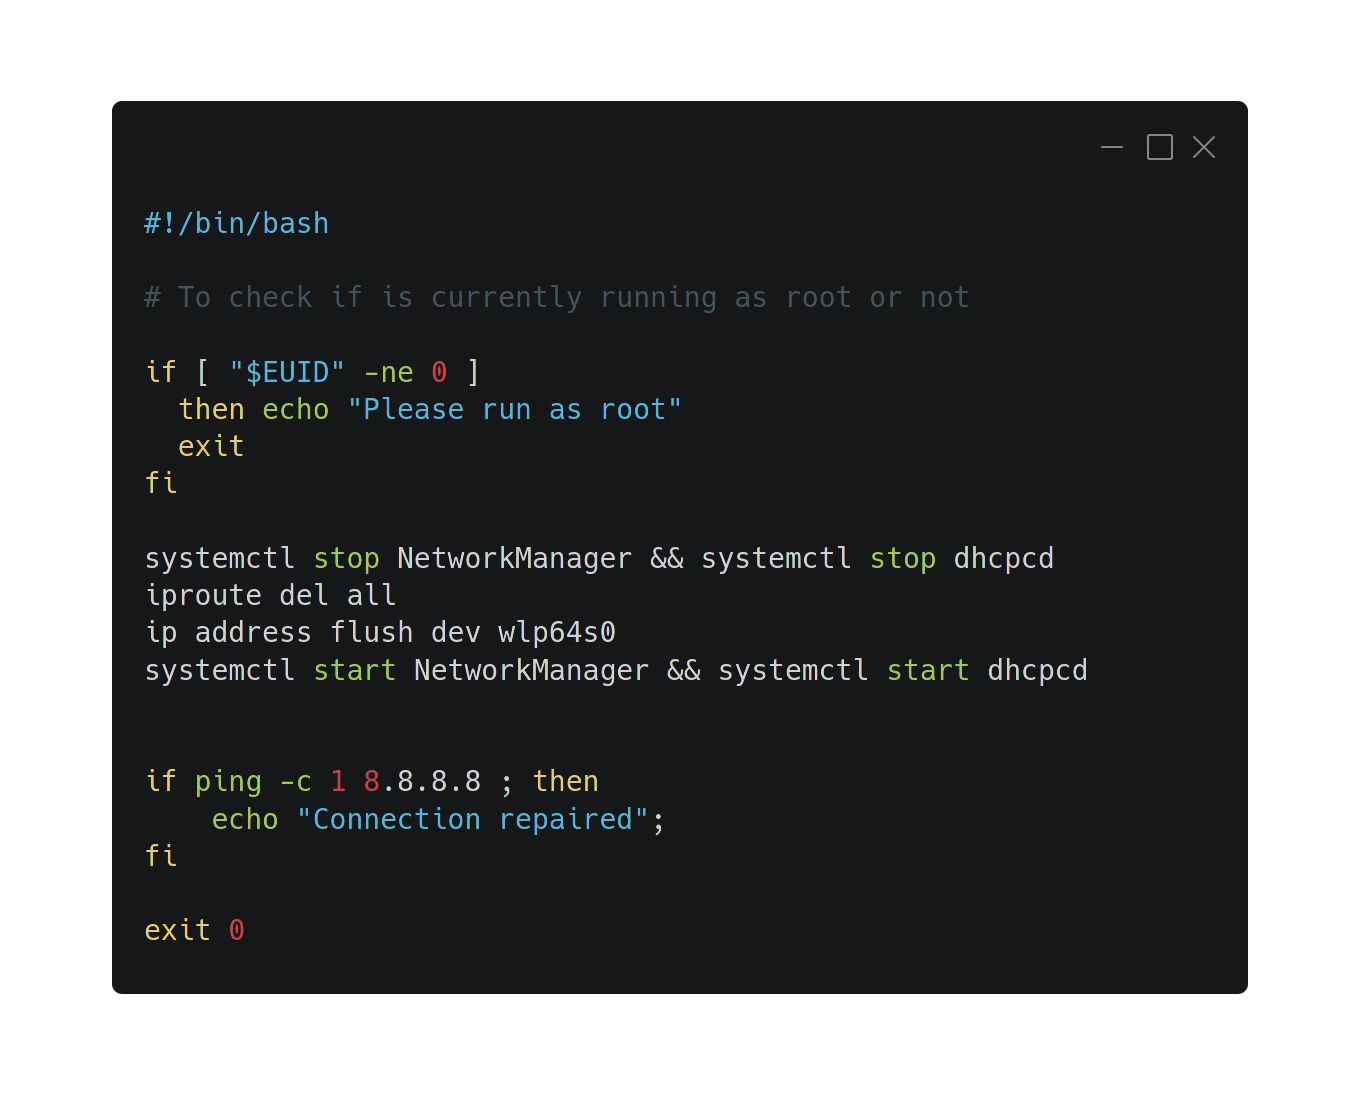
\includegraphics[width=\textwidth]{carbon.png}
\end{figure}

Gardez ce bout de code dans un coin, car ça m'a beaucoup aidé pour réparer automatiquement le "réseau" sur mon petit OS.
\\

On peut aussi afficher du "code" ou tout autre chose d'une façon "bloc note" avec ceci :
\begin{mycodebox}
    \begin{verbatim}
        message :  Q     B     I     T
        binary : 10000 00001 01000 10011
        Key :    11100 01011 01001 10010
        EncrB :  01100 00100 10010 00000
        EncrM :    M     I     S     A
    \end{verbatim}
\end{mycodebox}

Et si on a envie d'inclure directement un fichier \texttt{.txt}, on peut le faire !

\VerbatimInput{src/contents/quCR_CHSH_Measurement.txt}

On peut aussi choisir d'écrire directement du code insérer en ligne. Si je veux expliquer que
\incode{$x = y + 1$}, je peux.

